\chapter{Results}
\label{ChapterResults}
This chapter analyzes the results of our experiments.
We will divide our analysis as follows;
analysis for the results of the same classifier across different revealed percentages of data (chunks),
analysis for the results of different classifiers across the same revealed percentages of data (chunks)
and analysis for different classifiers and different percentages all together using the $F_{\beta}-measure$.
% could also be reorganized as results for testbed and results for recommender


% Models excluded due to performance
There were two classifiers that we excluded because they attained significantly inferior results compared to their published scores; these are KNNMSM and LS.
Specially on the InsectWingbeatSound data set, for which we attained a difference in performance of -45.71\% for KNNMSM and -20.71\% for LS than the results published by \cite{bagnall2017great}.


% Data sets that were not finished for remaining classifiers
For the remaining classifiers, not all of them were able to finish on all data sets within the time constraint.
Specially the multivariate archive, which was challenging for most of the algorithms in terms of memory and time complexity.
Our choice of adapting univariate classifiers for multivariate problems using column ensembling might have made things even more challenging;
because this technique fits for each dimension in the data sets a classifier, which is a memory and space extensive solution.
This was clearly evident for the runs as the number of dimensions of the data sets increased.

TSF was the most successful algorithm in finishing the biggest number of datasets. It was able to finish all the data sets from both archives, with the exception of FaceDetection only.
WEASEL was the second best, finishing all data sets from both archives, except for the largest three multivariate data sets; DuckDuckGeese, FaceDetection and PEMS-SF.
WEASEL is known for its quality and speed but not for scalability \cite{lucas2019proximity}, it failed these data sets due to out of memory errors.
CBoss failed to run on DuckDuckGeese, FaceDetection, PEMS-SF and MotorImagery within our time constraint.
ST is known to be one of the slowest algorithms, but we use an enhanced version to accelerate its performance. However, ST was not able to finish within our time limit on 15 multivariate datasets; due to its linear time complexity with the number of dimensions. It hit the limit of the time constraint once the number dimensions reached 6.
%ERing,BasicMotions,Cricket,LSST,RacketSports,SelfRegulationSCP1,SelfRegulationSCP2,HandMovementDirection,NATOPS
%FingerMovements,Heartbeat,MotorImagery,FaceDetection,PEMS-SF,DuckDuckGeese
It has also failed on the Fungi dataset, because it couldn't find high quality shapelets during the contract time that we cofigured it to use.
The slowest of all and which achieved the least progress on the data sets was PForest. It finished a total of 7 multivariate data Sets and 35 univariate data sets.
Although PForest can attain quasi linear training times with the size of training data, but it has a training complexity, which can be quadratic with length based on its randomly selected distance measure.
This is why PForest hit the time contraint easily as the length of the time series increased.
All 5 classifiers completed 36 common data sets. TSF, WEASEL and CBoss finished more than 72 data sets, ST finished 61 data sets and PForest finished 42 data sets.

Table \ref{tab:longresults} presents the results of our experiments for the used 5 classifiers on all 77 data sets.
We display values for balanced accuracy, $F_{\beta}-measure$ value and revealed\% for each classifier.
The default train/test split of the data sets was used for all data runs.

\begin{tiny}
    \begin{landscape}
    \begin{longtable}{|l|llll|llll|llll|llll|llll|}
        \caption{$F_{\beta}$ scores for all 5 classifiers on 77 data sets for all chunks} \label{tab:longresults} \\
        \hline
        \multirow{2}{*}{\textbf{Data set}} & 
        \multicolumn{4}{c}{\textbf{CBoss}} & \multicolumn{4}{c}{\textbf{PForest}} & \multicolumn{4}{c}{\textbf{ST}} & \multicolumn{4}{c}{\textbf{TSF}} & \multicolumn{4}{c}{\textbf{WEASEL}} \\
        & \textbf{10\%} & \textbf{20\%} & \textbf{30\%} & \textbf{100\%} & \textbf{10\%} & \textbf{20\%} & \textbf{30\%} & \textbf{100\%} & \textbf{10\%} & \textbf{20\%} & \textbf{30\%} & \textbf{100\%} & \textbf{10\%} & \textbf{20\%} & \textbf{30\%} & \textbf{100\%} & \textbf{10\%} & \textbf{20\%} & \textbf{30\%} & \textbf{100\%} \\ [0.5ex]
        \hline
        \endfirsthead % <-- This denotes the end of the header, which will be shown on the first page only
        \hline
        \multirow{2}{*}{\textbf{Data set}} & 
        \multicolumn{4}{c}{\textbf{CBoss}} & \multicolumn{4}{c}{\textbf{PForest}} & \multicolumn{4}{c}{\textbf{ST}} & \multicolumn{4}{c}{\textbf{TSF}} & \multicolumn{4}{c}{\textbf{WEASEL}} \\
        & \textbf{10\%} & \textbf{20\%} & \textbf{30\%} & \textbf{100\%} & \textbf{10\%} & \textbf{20\%} & \textbf{30\%} & \textbf{100\%} & \textbf{10\%} & \textbf{20\%} & \textbf{30\%} & \textbf{100\%} & \textbf{10\%} & \textbf{20\%} & \textbf{30\%} & \textbf{100\%} & \textbf{10\%} & \textbf{20\%} & \textbf{30\%} & \textbf{100\%} \\ [0.5ex]
        \hline
        \endhead % <-- Everything between \endfirsthead and \endhead will be shown as a header on every page
        ACSF1 & 0.7778 & 0.7477 & 0.7081 & 0.8780 & 0.6527 & 0.4819 & 0.3780 &  & 0.8030 & 0.8163 & 0.8433 & 0.7847 & 0.7740 & 0.6838 & 0.6613 & 0.5977 & 0.7899 & 0.7619 & 0.6842 & 0.8900  \\[1ex]
        \hline
        AtrialFibrillation & 0.6667 & 0.4800 & 0.4310 & 0.1667 & 0.7000 & 0.6000 & 0.4000 & 0.2857 & 0.7143 & 0.4800 & 0.5385 & 0.3478 & 0.6667 & 0.5455 & 0.3438 & 0.2254 & 0.7143 & 0.5455 & 0.4310 & 0.2254  \\[1ex]
        \hline
        BasicMotions & 0.7105 & 0.8421 & 1.0000 & 1.0000 & 0.6739 & 0.6154 & 0.5588 & 0.7059 &  &  &  &  & 0.8200 & 0.9697 & 1.0000 & 1.0000 & 0.7500 & 1.0000 & 1.0000 & 1.0000  \\[1ex]
        \hline
        Beef & 0.6765 & 0.5000 & 0.5800 & 0.7619 & 0.6714 & 0.5106 & 0.3710 & 0.2553 & 0.6667 & 0.5581 & 0.5385 & 0.7619 & 0.7857 & 0.7273 & 0.7273 & 0.6512 & 0.6579 & 0.5106 & 0.5000 & 0.7619  \\[1ex]
        \hline
        Car & 0.6846 & 0.5393 & 0.5189 & 0.8000 & 0.7143 & 0.5333 & 0.4474 & 0.4280 & 0.6875 & 0.5926 & 0.6134 & 0.7809 & 0.7500 & 0.7164 & 0.6613 & 0.6693 & 0.6846 & 0.5393 & 0.4558 & 0.8387  \\[1ex]
        \hline
        Chinatown & 0.6388 & 0.6526 & 0.7110 & 0.9388 & 0.6548 & 0.5484 & 0.9748 & 0.9674 & 0.6630 & 0.7311 & 0.7293 & 0.9638 & 0.9561 & 0.9820 & 0.9784 & 0.9566 & 0.6388 & 0.4742 & 0.3912 & 0.9353  \\[1ex]
        \hline
        CinCECGTorso & 0.6854 & 0.5433 & 0.4528 & 0.7578 &  &  &  &  & 0.6752 & 0.5562 & 0.5606 & 0.8988 & 0.7235 & 0.6748 & 0.7358 & 0.8876 & 0.7616 & 0.8160 & 0.6891 & 0.9516  \\[1ex]
        \hline
        Coffee & 0.7314 & 0.9573 & 0.9566 & 1.0000 & 0.7642 & 0.6512 & 0.7115 & 1.0000 & 0.7917 & 0.8485 & 0.9566 & 0.9123 & 0.8944 & 0.8485 & 0.8057 & 1.0000 & 0.7314 & 0.9180 & 0.6560 & 1.0000  \\[1ex]
        \hline
        Computers & 0.7717 & 0.7168 & 0.6811 & 0.6425 & 0.7427 & 0.6289 & 0.5714 & 0.5537 & 0.7525 & 0.6780 & 0.6628 & 0.6382 & 0.7841 & 0.7299 & 0.7097 & 0.6642 & 0.7193 & 0.7042 & 0.7032 & 0.6729  \\[1ex]
        \hline
        Cricket & 0.6569 & 0.7423 & 0.8171 & 1.0000 &  &  &  &  &  &  &  &  & 0.8445 & 0.8521 & 0.9179 & 0.8980 & 0.7156 & 0.6575 & 0.7781 & 0.9827  \\[1ex]
        \hline
        Earthquakes & 0.8068 & 0.7606 & 0.7398 & 0.7039 & 0.8068 & 0.7606 & 0.7398 & 0.7119 & 0.7536 & 0.7606 & 0.7398 & 0.5950 & 0.8068 & 0.7606 & 0.7398 & 0.7039 & 0.8068 & 0.7554 & 0.7337 & 0.7039  \\[1ex]
        \hline
        ECG200 & 0.6942 & 0.5674 & 0.4778 & 0.7962 & 0.7667 & 0.7767 & 0.5483 & 0.8780 & 0.7632 & 0.8081 & 0.7575 & 0.8309 & 0.8448 & 0.8511 & 0.8632 & 0.8193 & 0.7439 & 0.5926 & 0.5119 & 0.8193  \\[1ex]
        \hline
        ECG5000 & 0.6912 & 0.6739 & 0.8134 & 0.9283 & 0.7469 & 0.6585 & 0.6137 & 0.5533 & 0.8147 & 0.8715 & 0.8973 & 0.9248 & 0.9219 & 0.9123 & 0.9026 & 0.9218 & 0.7410 & 0.8070 & 0.7452 & 0.9264  \\[1ex]
        \hline
        ECGFiveDays & 0.7441 & 0.6168 & 0.5606 & 1.0000 & 0.7286 & 0.6543 & 0.6006 & 0.8208 & 0.7229 & 0.6734 & 0.6521 & 0.9985 & 0.7516 & 0.6728 & 0.6213 & 0.9032 & 0.7320 & 0.6315 & 0.5882 & 0.9985  \\[1ex]
        \hline
        ElectricDevices & 0.7024 & 0.5731 & 0.5578 & 0.6558 &  &  &  &  & 0.6961 & 0.5575 & 0.4304 & 0.3292 & 0.7315 & 0.6354 & 0.6122 & 0.6355 & 0.7513 & 0.6637 & 0.6086 & 0.7262  \\[1ex]
        \hline
        EOGHorizontalSignal & 0.6506 & 0.4682 & 0.4058 & 0.4200 & 0.6509 & 0.4614 & 0.3393 &  & 0.6522 & 0.4659 & 0.4058 & 0.4173 & 0.6544 & 0.4659 & 0.3958 & 0.4581 & 0.6496 & 0.4743 & 0.3672 & 0.4227  \\[1ex]
        \hline
        EOGVerticalSignal & 0.6538 & 0.4704 & 0.3777 & 0.3693 &  &  &  &  & 0.6506 & 0.4674 & 0.4095 & 0.3353 & 0.6525 & 0.4682 & 0.4045 & 0.3985 & 0.6490 & 0.4674 & 0.3513 & 0.2714  \\[1ex]
        \hline
        Epilepsy & 0.9662 & 1.0000 & 1.0000 & 1.0000 &  &  &  &  & 0.7993 & 0.7920 & 0.8678 & 0.9819 & 0.9169 & 0.9735 & 0.9733 & 0.9640 & 0.9825 & 1.0000 & 1.0000 & 1.0000  \\[1ex]
        \hline
        ERing & 0.6800 & 0.5340 & 0.5135 & 0.8736 & 0.6617 & 0.5015 & 0.4061 & 0.4518 &  &  &  &  & 0.7547 & 0.7689 & 0.8266 & 0.9405 & 0.6856 & 0.5820 & 0.5876 & 0.9405  \\[1ex]
        \hline
        EthanolConcentration & 0.6741 & 0.5127 & 0.4235 & 0.3579 &  &  &  &  & 0.6954 & 0.5590 & 0.4729 & 0.5541 & 0.7045 & 0.5838 & 0.4996 & 0.3688 & 0.6770 & 0.5177 & 0.4649 & 0.5073  \\[1ex]
        \hline
        EthanolLevel & 0.6779 & 0.5181 & 0.4346 & 0.3937 &  &  &  &  & 0.6866 & 0.5618 & 0.4719 & 0.3085 & 0.6942 & 0.5464 & 0.4554 & 0.3937 & 0.6742 & 0.5168 & 0.4240 & 0.4385  \\[1ex]
        \hline
        FingerMovements & 0.7105 & 0.6202 & 0.5526 & 0.5147 &  &  &  &  &  &  &  &  & 0.7062 & 0.6250 & 0.5588 & 0.4444 & 0.7247 & 0.6202 & 0.5588 & 0.5351  \\[1ex]
        \hline
        FordA & 0.8003 & 0.8341 & 0.8237 & 0.6833 &  &  &  &  & 0.7087 & 0.6150 & 0.5944 & 0.4967 & 0.7940 & 0.7570 & 0.7585 & 0.7774 & 0.8329 & 0.7970 & 0.9160 & 0.9577  \\[1ex]
        \hline
        FordB & 0.7765 & 0.7465 & 0.7232 & 0.5672 &  &  &  &  & 0.7285 & 0.6017 & 0.6037 & 0.4813 & 0.7488 & 0.6722 & 0.6400 & 0.6352 & 0.7630 & 0.7696 & 0.6417 & 0.7830  \\[1ex]
        \hline
        FreezerRegularTrain & 0.7222 & 0.9715 & 0.9987 & 0.9956 & 0.7890 & 0.6250 & 0.8963 & 0.9049 & 0.7237 & 0.9433 & 0.9987 & 0.9987 & 0.9645 & 0.9982 & 0.9982 & 0.9891 & 0.7222 & 0.9287 & 0.7329 & 0.9751  \\[1ex]
        \hline
        FreezerSmallTrain & 0.7226 & 0.9457 & 0.9974 & 0.9656 & 0.7518 & 0.6360 & 0.7200 & 0.6611 & 0.7191 & 0.9127 & 0.9982 & 0.9996 & 0.8893 & 0.9798 & 0.9978 & 0.8085 & 0.7222 & 0.8955 & 0.6456 & 0.9505  \\[1ex]
        \hline
        Fungi & 0.6516 & 0.4553 & 0.3324 &  & 0.6492 & 0.4757 & 0.4373 & 0.8947 &  &  &  &  & 0.6554 & 0.5280 & 0.5489 & 0.9337 & 0.6486 & 0.4595 & 0.3429 & 0.9468  \\[1ex]
        \hline
        Ham & 0.7188 & 0.6131 & 0.5500 & 0.6154 & 0.7211 & 0.6269 & 0.5559 & 0.6563 & 0.7188 & 0.6087 & 0.5800 & 0.7191 & 0.7471 & 0.7636 & 0.7273 & 0.7404 & 0.7258 & 0.6222 & 0.5500 & 0.5952  \\[1ex]
        \hline
        HandMovementDirection & 0.6814 & 0.5008 & 0.4328 & 0.3149 & 0.6670 & 0.5184 & 0.4737 & 0.3275 &  &  &  &  & 0.6770 & 0.5421 & 0.4394 & 0.4985 & 0.6729 & 0.5008 & 0.3892 & 0.3149  \\[1ex]
        \hline
        Handwriting & 0.6469 & 0.4449 & 0.3753 & 0.4110 &  &  &  &  & 0.6469 & 0.4465 & 0.3596 & 0.3114 & 0.6570 & 0.4952 & 0.4341 & 0.2649 & 0.6471 & 0.4416 & 0.3338 & 0.2639  \\[1ex]
        \hline
        HouseTwenty & 0.7172 & 0.7855 & 0.8489 & 0.9687 & 0.8190 & 0.7544 & 0.7184 & 0.8770 & 0.7627 & 0.7791 & 0.8239 & 0.8081 & 0.8628 & 0.9225 & 0.8927 & 0.7791 & 0.8864 & 0.9407 & 0.9204 & 0.9583  \\[1ex]
        \hline
        InsectEPGRegularTrain & 0.9672 & 0.9432 & 1.0000 & 1.0000 & 1.0000 & 0.9950 & 1.0000 & 1.0000 & 0.6918 & 0.5592 & 0.4855 & 0.9850 & 1.0000 & 1.0000 & 1.0000 & 1.0000 & 1.0000 & 1.0000 & 1.0000 & 1.0000  \\[1ex]
        \hline
        InsectEPGSmallTrain & 0.9129 & 1.0000 & 0.9467 & 1.0000 & 0.9950 & 0.9005 & 0.9851 & 1.0000 & 0.6918 & 0.5577 & 0.4833 & 0.9651 & 1.0000 & 1.0000 & 1.0000 & 1.0000 & 1.0000 & 1.0000 & 1.0000 & 1.0000  \\[1ex]
        \hline
        InsectWingbeatSound & 0.6522 & 0.4898 & 0.4517 & 0.4964 &  &  &  &  & 0.6521 & 0.4851 & 0.3914 & 0.5654 & 0.7115 & 0.6489 & 0.6383 & 0.5633 & 0.6566 & 0.5333 & 0.4813 & 0.5839  \\[1ex]
        \hline
        ItalyPowerDemand & 0.6943 & 0.5766 & 0.7891 & 0.8641 & 0.7071 & 0.7106 & 0.5802 & 0.9495 & 0.6866 & 0.5852 & 0.6913 & 0.9447 & 0.7592 & 0.7142 & 0.7609 & 0.9531 & 0.6943 & 0.5841 & 0.5566 & 0.9117  \\[1ex]
        \hline
        LargeKitchenAppliances & 0.7273 & 0.6186 & 0.5714 & 0.7289 & 0.6979 & 0.5607 & 0.5045 & 0.3783 & 0.6904 & 0.5495 & 0.4726 & 0.6154 & 0.7212 & 0.6061 & 0.5417 & 0.5154 & 0.6816 & 0.5405 & 0.4629 & 0.6382  \\[1ex]
        \hline
        Libras & 0.6241 & 0.4404 & 0.4136 & 0.7936 & 0.6269 & 0.4274 & 0.3238 & 0.0541 & 0.6299 & 0.4524 & 0.3966 & 0.8387 & 0.6790 & 0.6465 & 0.6853 & 0.7682 & 0.6352 & 0.4898 & 0.5078 & 0.8387  \\[1ex]
        \hline
        Lightning2 & 0.7328 & 0.6438 & 0.5850 & 0.6923 & 0.7089 & 0.6612 & 0.5850 & 0.8031 & 0.7328 & 0.5966 & 0.5537 & 0.6565 & 0.7328 & 0.6893 & 0.7039 & 0.6565 & 0.7328 & 0.6612 & 0.6414 & 0.6212  \\[1ex]
        \hline
        Lightning7 & 0.6941 & 0.5541 & 0.5218 & 0.6945 & 0.6619 & 0.4974 & 0.3963 & 0.2566 & 0.6584 & 0.4771 & 0.4280 & 0.6497 & 0.6755 & 0.6186 & 0.5896 & 0.6945 & 0.6867 & 0.5242 & 0.4150 & 0.6795  \\[1ex]
        \hline
        LSST & 0.6241 & 0.5174 & 0.4533 & 0.4529 &  &  &  &  &  &  &  &  & 0.6885 & 0.5777 & 0.5268 & 0.4489 & 0.6823 & 0.5844 & 0.5108 & 0.5318  \\[1ex]
        \hline
        Meat & 0.8636 & 0.7059 & 0.8500 & 0.8583 & 0.7353 & 0.5714 & 0.4643 & 0.5977 & 0.8077 & 0.9231 & 0.8012 & 0.9587 & 0.8333 & 0.8276 & 0.8333 & 0.9180 & 0.7609 & 0.6154 & 0.4643 & 0.8193  \\[1ex]
        \hline
        MoteStrain & 0.7139 & 0.7458 & 0.6324 & 0.9320 & 0.7060 & 0.7817 & 0.7693 & 0.8688 & 0.7341 & 0.5966 & 0.7172 & 0.8992 & 0.8789 & 0.8666 & 0.8698 & 0.8452 & 0.7716 & 0.7817 & 0.7946 & 0.9418  \\[1ex]
        \hline
        NATOPS & 0.6469 & 0.5186 & 0.4640 & 0.8000 & 0.6376 & 0.4753 & 0.3795 & 0.1860 &  &  &  &  & 0.6443 & 0.5207 & 0.5171 & 0.7682 & 0.6426 & 0.5269 & 0.5407 & 0.8000  \\[1ex]
        \hline
        NonInvasiveFetalECGThorax1 & 0.7116 & 0.5647 & 0.6373 & 0.7851 &  &  &  &  & 0.7298 & 0.7056 & 0.6204 & 0.2848 & 0.8362 & 0.7959 & 0.7829 & 0.8453 & 0.6454 & 0.4942 & 0.4060 &   \\[1ex]
        \hline
        NonInvasiveFetalECGThorax2 & 0.6838 & 0.7068 & 0.5754 & 0.8227 &  &  &  &  & 0.6795 & 0.7408 & 0.7543 & 0.5136 & 0.8697 & 0.8353 & 0.8052 & 0.8784 & 0.6453 & 0.4637 & 0.3614 & 0.9045  \\[1ex]
        \hline
        OliveOil & 0.6935 & 0.8571 & 0.9211 & 0.8387 & 0.6667 & 0.5000 & 0.5000 & 0.5113 & 0.7727 & 0.9231 & 0.8846 & 0.8780 & 0.8000 & 0.8000 & 0.8846 & 0.8387 & 0.6579 & 0.4898 & 0.4474 & 0.8780  \\[1ex]
        \hline
        Phoneme & 0.6627 & 0.5061 & 0.4238 & 0.2683 & 0.6443 & 0.4479 & 0.3233 & 0.0135 & 0.6647 & 0.5018 & 0.4130 & 0.2345 & 0.6576 & 0.4936 & 0.3978 & 0.1652 & 0.6684 & 0.5135 & 0.4360 & 0.2578  \\[1ex]
        \hline
        PigAirwayPressure & 0.6605 & 0.5082 & 0.4185 & 0.9115 &  &  &  &  & 0.6581 & 0.5006 & 0.5130 & 0.7543 & 0.6534 & 0.4722 & 0.3517 & 0.1851 & 0.6807 & 0.5730 & 0.4968 & 0.5865  \\[1ex]
        \hline
        PigArtPressure & 0.9771 & 0.9940 & 0.9822 & 0.9761 &  &  &  &  & 0.8881 & 0.9073 & 0.9534 & 0.9524 & 0.6624 & 0.5067 & 0.4369 & 0.3515 & 0.9370 & 0.9652 & 0.9591 & 1.0000  \\[1ex]
        \hline
        PigCVP & 0.8077 & 0.8786 & 0.9257 & 0.9406 & 0.6443 & 0.4529 &  &  & 0.6881 & 0.5892 & 0.7251 & 0.7219 & 0.6599 & 0.4903 & 0.3880 & 0.2363 & 0.7142 & 0.6809 & 0.8155 & 0.9173  \\[1ex]
        \hline
        Plane & 0.6721 & 0.4884 & 0.5223 & 1.0000 & 0.6909 & 0.5316 & 0.5637 & 1.0000 & 0.6736 & 0.6316 & 0.6357 & 1.0000 & 0.9118 & 0.9767 & 0.9538 & 0.9881 & 0.6615 & 0.4884 & 0.8692 & 1.0000  \\[1ex]
        \hline
        PowerCons & 0.7432 & 0.7164 & 0.7595 & 0.9046 & 0.7647 & 0.6792 & 0.6847 & 0.9931 & 0.7368 & 0.6180 & 0.6673 & 0.9248 & 0.8103 & 0.7742 & 0.7796 & 0.9931 & 0.7323 & 0.6457 & 0.6259 & 0.9519  \\[1ex]
        \hline
        RacketSports & 0.6749 & 0.5096 & 0.4389 & 0.7724 & 0.6914 & 0.5319 & 0.4654 & 0.3804 &  &  &  &  & 0.7517 & 0.7255 & 0.7821 & 0.8796 & 0.6914 & 0.5588 & 0.5232 & 0.8485  \\[1ex]
        \hline
        RefrigerationDevices & 0.7280 & 0.6000 & 0.5647 & 0.4883 & 0.7000 & 0.5848 & 0.5530 & 0.4066 & 0.7246 & 0.6036 & 0.5714 & 0.5045 & 0.7294 & 0.6329 & 0.5800 & 0.5317 & 0.6969 & 0.5792 & 0.5290 & 0.4484  \\[1ex]
        \hline
        Rock & 0.7083 & 0.5882 & 0.6111 & 0.8780 & 0.6818 & 0.5333 & 0.4278 & 0.4053 & 0.6754 & 0.5128 & 0.4474 & 0.8544 & 0.7174 & 0.6452 & 0.6392 & 0.6948 & 0.6724 & 0.5797 & 0.3911 & 0.7619  \\[1ex]
        \hline
        ScreenType & 0.7016 & 0.5859 & 0.5212 & 0.4379 & 0.6933 & 0.5405 &  &  & 0.6908 & 0.5682 & 0.5045 & 0.4300 & 0.6989 & 0.5780 & 0.5258 & 0.3808 & 0.7101 & 0.5758 & 0.5227 & 0.4776  \\[1ex]
        \hline
        SelfRegulationSCP1 & 0.7614 & 0.7052 & 0.6862 & 0.7449 &  &  &  &  &  &  &  &  & 0.8097 & 0.8389 & 0.8265 & 0.7604 & 0.7673 & 0.8637 & 0.7845 & 0.7604  \\[1ex]
        \hline
        SelfRegulationSCP2 & 0.7209 & 0.6400 & 0.6211 & 0.4720 & 0.7081 &  &  &  &  &  &  &  & 0.7293 & 0.6316 & 0.5836 & 0.4226 & 0.7209 & 0.6316 & 0.6172 & 0.5512  \\[1ex]
        \hline
        SemgHandGenderCh2 & 0.7810 & 0.6957 & 0.7602 & 0.8563 &  &  &  &  & 0.6911 & 0.7090 & 0.8235 & 0.7752 & 0.8150 & 0.8905 & 0.8758 & 0.9120 & 0.7667 & 0.7007 & 0.6625 & 0.7487  \\[1ex]
        \hline
        SemgHandMovementCh2 & 0.6633 & 0.4898 & 0.3921 & 0.5918 &  &  &  &  & 0.6689 & 0.5573 & 0.4747 & 0.4183 & 0.7356 & 0.6792 & 0.7126 & 0.8128 & 0.6633 & 0.4898 & 0.3960 & 0.2513  \\[1ex]
        \hline
        SemgHandSubjectCh2 & 0.6789 & 0.5165 & 0.4914 & 0.7096 &  &  &  &  & 0.6837 & 0.6218 & 0.6172 & 0.5272 & 0.7586 & 0.7826 & 0.7696 & 0.8940 & 0.6667 & 0.5000 & 0.4529 & 0.5872  \\[1ex]
        \hline
        SmallKitchenAppliances & 0.7964 & 0.7353 & 0.6842 & 0.7378 & 0.6938 & 0.5837 & 0.4854 &  & 0.7113 & 0.5535 & 0.5321 & 0.7408 & 0.7727 & 0.7059 & 0.6638 & 0.7954 & 0.7435 & 0.7026 & 0.5870 & 0.6729  \\[1ex]
        \hline
        SonyAIBORobotSurface1 & 0.7228 & 0.8016 & 0.5272 & 0.4126 & 0.8168 & 0.8307 & 0.8485 & 0.7908 & 0.7060 & 0.7104 & 0.7017 & 0.9202 & 0.7873 & 0.7720 & 0.7460 & 0.6445 & 0.7212 & 0.8841 & 0.8621 & 0.8003  \\[1ex]
        \hline
        SonyAIBORobotSurface2 & 0.7000 & 0.6669 & 0.8502 & 0.8947 & 0.7547 & 0.6644 & 0.7324 & 0.8548 & 0.7554 & 0.6712 & 0.6401 & 0.8947 & 0.8088 & 0.7926 & 0.7785 & 0.7413 & 0.7973 & 0.7704 & 0.8981 & 0.9340  \\[1ex]
        \hline
        StandWalkJump & 0.7000 & 0.5000 & 0.4643 & 0.2857 & 0.6875 & 0.5217 & 0.4643 &  & 0.6875 & 0.5714 & 0.4643 & 0.2857 & 0.7143 & 0.5455 & 0.5385 & 0.3478 & 0.7143 & 0.5714 & 0.5800 & 0.2857  \\[1ex]
        \hline
        StarlightCurves & 0.6805 & 0.5271 & 0.4523 & 0.9688 &  &  &  &  & 0.7431 & 0.6986 & 0.7900 & 0.9151 & 0.9250 & 0.9413 & 0.9521 & 0.9528 & 0.6911 & 0.5294 & 0.4376 & 0.9375  \\[1ex]
        \hline
        Strawberry & 0.7643 & 0.6916 & 0.9573 & 0.9698 & 0.7643 & 0.6916 & 0.6563 & 0.9039 & 0.8033 & 0.7769 & 0.7686 & 0.9268 & 0.8957 & 0.9024 & 0.9478 & 0.9366 & 0.7643 & 0.6916 & 0.6563 & 0.9565  \\[1ex]
        \hline
        Trace & 0.6835 & 0.5755 & 0.7000 & 1.0000 & 0.7273 & 0.6154 & 0.5465 & 0.4743 & 0.6818 & 0.5063 & 0.3955 & 1.0000 & 0.7740 & 0.7339 & 0.6842 & 0.9875 & 0.6724 & 0.5442 & 0.5000 & 1.0000  \\[1ex]
        \hline
        TwoLeadECG & 0.7236 & 0.6084 & 0.6552 & 0.9956 & 0.7581 & 0.7010 & 0.6714 & 0.9307 & 0.7223 & 0.6176 & 0.6357 & 0.9978 & 0.8011 & 0.8276 & 0.9348 & 0.7018 & 0.7223 & 0.6230 & 0.6493 & 0.9978  \\[1ex]
        \hline
        UWaveGestureLibrary & 0.6546 & 0.4839 & 0.3930 & 0.8157 &  &  &  &  & 0.6569 & 0.4776 & 0.3688 & 0.8595 & 0.7006 & 0.6772 & 0.7101 & 0.8193 & 0.6524 & 0.4971 & 0.4290 & 0.7761  \\[1ex]
        \hline
        Wafer & 0.9271 & 0.9807 & 0.9847 & 0.9961 & 0.9319 & 0.9500 & 0.8955 & 0.9935 & 0.9450 & 1.0000 & 0.9949 & 1.0000 & 0.9948 & 0.9906 & 0.9931 & 0.9931 & 0.9932 & 0.8810 & 0.8763 & 0.9996  \\[1ex]
        \hline
        Wine & 0.7596 & 0.6334 & 0.7180 & 0.6957 & 0.7177 & 0.6429 & 0.7030 & 0.5378 & 0.7477 & 0.6526 & 0.6599 & 0.7162 & 0.7727 & 0.6626 & 0.6198 & 0.6753 & 0.7222 & 0.6154 & 0.6071 & 0.7577  \\[1ex]
        \hline
    %\end{longtabu}
    \end{longtable}
    \end{landscape}
  \end{tiny}

We divide our analysis into three parts: a comparison of the effect of data chopping within the same classifier,
comparison on the effect of data chopping across different classifiers and unified comparison between all classifiers
across all data chops.
Since some of the analysis results we present include comparisons between the same classifier trained on different percentages of data, we use a special naming convention.
We name the classifiers using the format $NameOfClassifier\_Revealed\%$, where the first part of the name refer to the name of the classifier
and the second part refers to the percentage of data used to train the classifier. For example, $TSF\_10$ refers to classifier TSF which was trained on 10\% of the data length.
This naming convention helps clarify the type of the classifier and the context of comparison regardless of the type of analysis being discussed.


\section{Results Across Classifiers}
\label{SectionAcrossComparison}
An aspect to investigate within the early classification context is the relative performance of classifiers to each other while more data becomes available to train on.
We fix the percentage of data revealed, revealed\%, and compare the performance of classifiers, which is represented by their ranking based on the value of $F_{\beta}-measure$.
We will dig deeper into the properties of the data sets, to explore the relation between the characteristics of the data and the best performing algorithm.

To better understand the actual performance of the classifiers on the data sets and assess the quality of their results, we introduce a new baseline classifier to the comparison.
The baseline classifier always predicts the majority class of a given data set.
We name the classifier \emph{dummy}; as an indication of its role in the comparisons.
To ensure the integrity of our comparisons, we calculate balanced accuracy and $F_{\beta}-measure$ for the dummy classifier on all data sets and for the same 4 chunks.
Although the dummy classifier will always predict the majority class and thus score the same balanced accuracy, but its $F_{\beta}-measure$ will differ based on the revealed\%.

Figure \ref{fig:CDAcross} shows the critical difference diagram across all the classifiers and for a fixed revealed percentage of data.
In the beginning when only 10\% of the data is revevaled, TSF is significantly better than all the other classifiers.
The remaining four classifiers form a clique together and are not significantly different from the dummy classifier.
Inside that clique, CBoss is the best classifier, WEASEL is the second best and both PForest and ST are almost identical in their ranking.

\begin{figure}
    \captionsetup{justification=raggedright}
    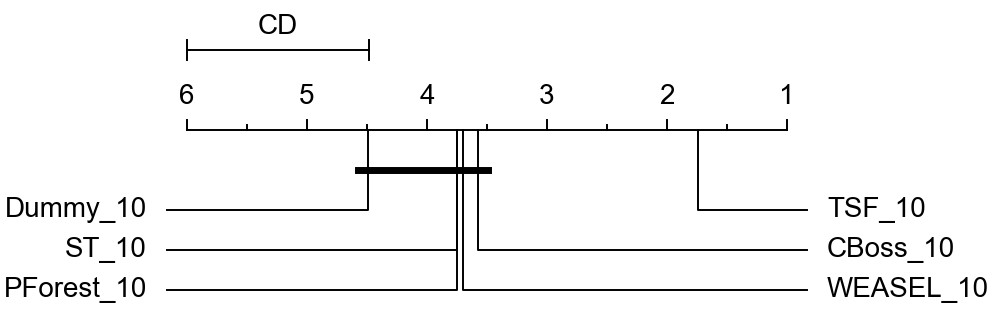
\includegraphics[width=0.49\textwidth,keepaspectratio]{cd_hm_across_10pct_with_dummy.png}
    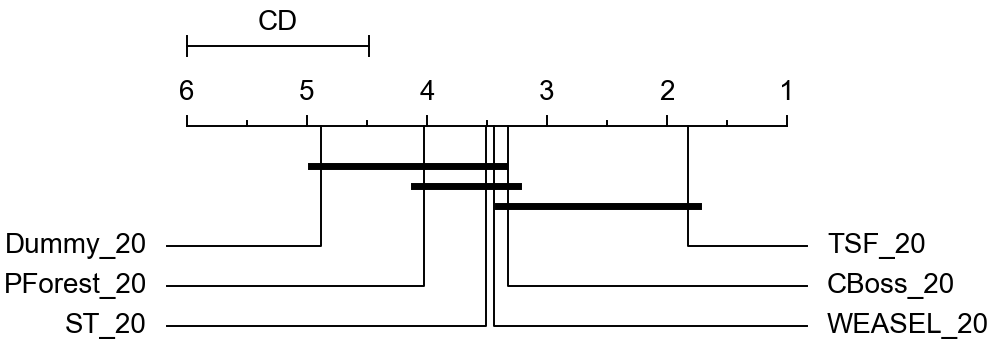
\includegraphics[width=0.49\textwidth,keepaspectratio]{cd_hm_across_20pct_with_dummy.png}
    \\[\smallskipamount]
    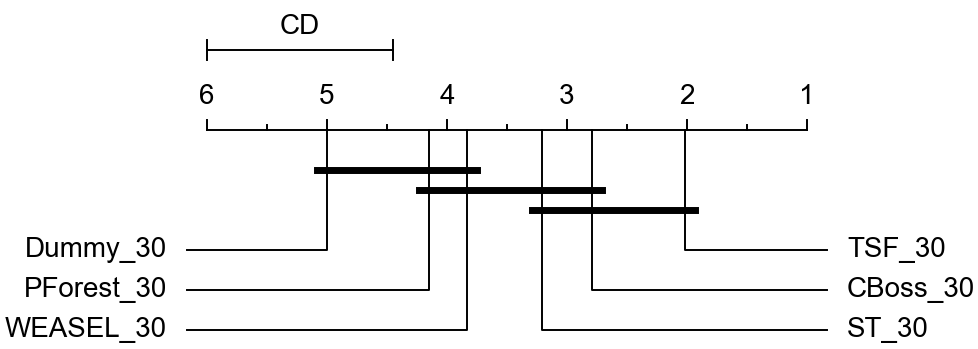
\includegraphics[width=0.49\textwidth,keepaspectratio]{cd_hm_across_30pct_with_dummy.png}
    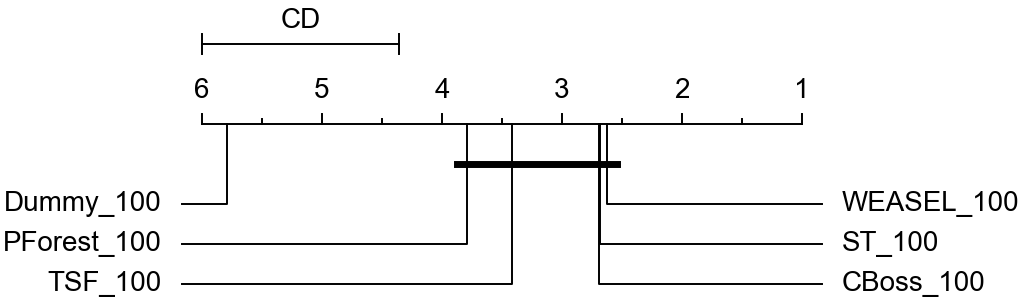
\includegraphics[width=0.49\textwidth,keepaspectratio]{cd_hm_across_100pct_with_dummy.png}
    \caption{Critical Difference diagrams per percentage across all classifiers}
    \label{fig:CDAcross}
\end{figure}

When the revealed percentage is increased to 20\%, TSF still prevails as the first classifier but with no significant different to CBoss and WEASEL.
There is still no significant difference between the PForest, ST and WEASEL and between the dummy classifier.
ST is able to learn better shapelets on the data and beats PForest.
On the third chunk, CBoss and ST are not significantly different from TSF and join it to form the first clique.
While WEASEL and PForest are not significantly different from the dummy classifier.
The middle clique shows no significant difference between CBoss, ST, WEASEL and PForest. However WEASEL and PForest are both significantly worse than TSF.
On the full length of data, the 5 classifiers are all not significantly different from each other.
WEASEL attains the best ranking followed by ST and CBoss which are identical, while TSF loses its edge on full length data.
PForest ranks the last among the 5 classifiers. All the classifiers form one clique which is significantly better than the dummy classifier.

The most apparent conclusion from the graphs is that TSF is able to do better on data sets during the earlier stages of the early classification context.
We believe the reason why TSF is always better on the shorter chunks of data; is because it uses three simple aggregations as features and doesn't depend on advanced features like the other classifiers do.
On the other side, the BOP technique applied by WEASEL and CBoss is challenged by the chopping, which notably decreases the chances of repetition of distinctive patterns in the data within such a small length.
PForest is also expected to perform badly as it needs to stretch the extent of its elastic distance measures; by measuring distances between testing instances which are 10$x$ the length of the training instances.
ST gets the lowest scores because in cases like our experiments where majority of the data is chopped, it is very hard to find shapelets that can uniquely indentify the different classes by learning on only the first 10\% of the data.
An obvious change is visible when more data is made available for training, the techniques of; WEASEL; CBoss and ST are able to make use of the more available information
to find better and more distinctive features in the data; which helps them be more competent.
Also PForest is able to score get better performances; because its elastic distance measure do not have to compensate for the big difference in length.


\section{Data Set characteristics and performance in early classification context}
\label{SectionDataCharacteristicsandPerformance}
The goal of our reasearch is to learn a recommender which can suggest the best classifiers to unseen data sets.
The recommender analyzes the characteristics of the data set and then based on the performance from previous experiments, it suggests the most suitable classifiers.
Thus it could be very convenient if the characteristics of the data sets we used; like length of series, number of classes and train size are able to provide insights about the best algorithm for a data set.
These comparison aspects were first defined in \cite{bagnall2017great} and have also been adopted in \cite{fawaz2019deepreview}.
The group of data sets we use for this analysis is very small and for some analysis we break them down by certain criteria.
We believe that our results should be interpreted carefully and not generalized for all data sets.

\subsection{Length of Series}
The first feature of the data sets we investigate is the length of the time series.
Like the findings of \cite{bagnall2017great} on univariate data sets and the results of \cite{fawaz2019deepreview} on multivariate data sets,
our results in the early classification context, didn't show information about the performance of the classifiers in accordance with the length of time series.
We show the results of the 5 classifiers on data sets grouped by their time series length in tables 123124 for the 10\% length, 123224234 for the 20\% length, 1242354235 for the 30\% length and 1242335 for the 100\% length.
The tables display for each classifier the total number of times it was able to score higher $F_{\beta}-measure$ than the baseline classifier.
In the case where multiple classifiers are able to score higher than the baseline on one data set, then the score of this data set is counted for each one of them.
We couldn't infer a strong relation between the length of time series and the performance of classifiers except for TSF. 
Our findings for TSF shows that it is consistently better than the baseline on all length groups for all data chunks.
It was able to score good results on all the data sets in the groups (51-100), (101-250) and (1001 +) even by training on only the 10\% chunk.
Unlike TSF, none of the other classifiers was able to beat the basline for the data set group with the least length (1-50).
There is a clear enhancement in the performance of all the classifiers as they learn on more data chunks as we have mentioned before,
but no clear relation between the length of the time series and the performance across the different chunks.

%Our findings for CBoss match the findings of \cite{bagnall2017great}; as the length of the time series increases CBoss shows better rankings.
%In the earlier context experiments when the data is chopped, CBoss couldn't score on any of the short length series and could hardly score on data sets of lengths more than 250.
%This improves as more data is made available for training and it completely dominates the longest length group on the 100\% length data.
%While PForest couldn't score at any of the experiments on the longest group of data sets.
%For the two earliest experiments; the 10\% and the 20\% chunks, our results comply with our findings from the critical difference diagrams.
%TFS dominates all other classifiers on all length groups, except for the group with the longest length where WEASEL shows more competence.


\subsection{Training Data Set Size}
The second feature of the data sets we investigate is the training size, and how the number of instances affects the performance of classifiers in our introduced context.
We display our results for the train size feature in tables; 123124 for the 10\% length, 123224234 for the 20\% length, 1242354235 for the 30\% length and 1242335 for the 100\% length.
The table displays for each classifier the total number of times a it was able to score higher than the baseline classifier.
TSF consistently scores better than, or at least the same as, the other classifiers on all train size groups for the first 3 chunks.
The scores for TSF on all the train size groups are better than the baseline across the different chunks except for the second group (51-100) on the 10\% chunk.
TSF levels with the baseline classifier on the two data sets Lightning2 and Lightning7 on thee 10\% chunk, but beats it once more data is available.
During the 20\% and the 30\% chunks, WEASEL cannot beat the baseline classifier on the data sets in the largest train size group.
However on the 100\% chunk it catches up and beats it on both data sets.
Our results don't show any significance from comparing algorithms based on the training size across the different early classification runs.
There is also no significance of patterns of the performance of the same classifiers.
%Yet there is an interesting pattern regarding the performance of WEASEL across the different experiments.
%WEASEL scores better performances on the small train size groups and worse on the bigger size data sets.
%This pattern is consistent on all the chunks.


\subsection{Type of Problem}
The third feature of the data sets we investigate is the type of problem.
The intention is to try to find an evidence if there is a classifier which is suitable for certain types of problems.
We display our results for the data set type feature in tables; 123124 for the 10\% length, 123224234 for the 20\% length, 1242354235 for the 30\% length and 1242335 for the 100\% length.
Our results show that TSF is able to achieve better results than the baseline classifier on all data sets of the type SPECTRO.
This performance is consistently kept across all the different chops, till the other classifiers catch up on the full length data chop.
PForest is not able to beat the baseline on types HAR and SOUND during any of the experiments.
However, since both types consist only of one data set, we cannot conclude that PForest will not be able to learn on such types.
During the full length experiment, all the classifiers are able to beat the baseline classifier on all the data sets for the groups; SPECTRO, Traffic, DEVICE and EPG.


\subsection{Number of classes}
The fourth feature of the data sets we investigate is the number of classes.
The goal is to try to find a connection between the number of classes of data sets and if it has an impact on the performance of certain classifiers.
We display our results for the number of classes feature in tables; 123124 for the 10\% length, 123224234 for the 20\% length, 1242354235 for the 30\% length and 1242335 for the 100\% length.
Like our previous observations for the other faetures, TSF is constantly better than the baseline classifier on all groups across all the chunks.
It starts with a good performance on all groups in the 10\% experiment and maintains a slight improvement till it reaches the 100\%.
PForest and ST generally perform better on data sets with small number of classes. As they move towards the 100\% chunk they tend to enhance their performance gradually.
WEASEL and CBoss on the contrary learn better on the data sets with larger number of classes at the earlier chunks.
PForest cannot beat the baseline classifier on the group of (11+) across all chunks. Since the group consists of only two data sets, we cannot generalize this conclusion.


\section{Results Within Classifier}
\label{SectionWithinComparison}
In our first experiment, we carry out a comparison between copies of the same classifier but trained using different chunks of data;
to explore how their performances evolve in the early classification context. We combine results that are based on both $F_{\beta}-measure$ and balanced accuracy.
We exclude the baseline classifier from this comparison.


\begin{figure} [H]
    \centering
    \begin{tabular}{ccc}
    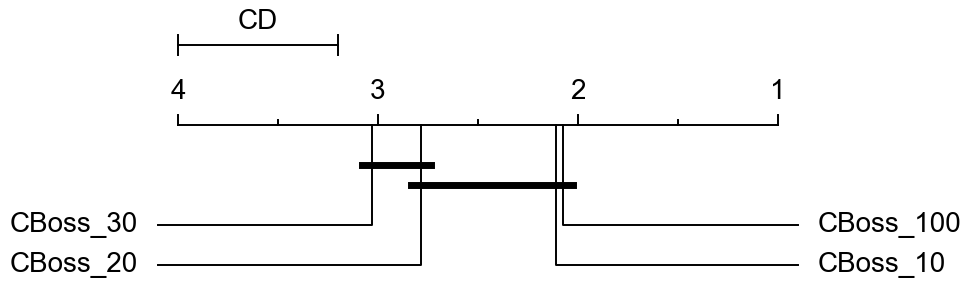
\includegraphics[width=0.49\textwidth]{cd_hm_within_cboss.png} & & 
    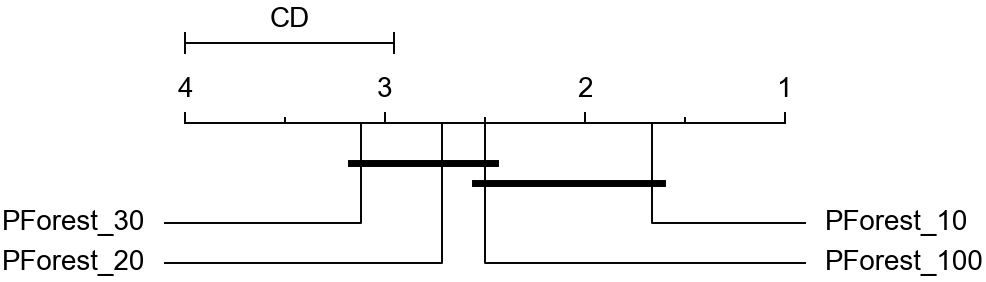
\includegraphics[width=0.40\textwidth]{cd_hm_within_pforest.png} \\
    \textbf{(a)} & & \textbf{(b)} \\[6pt]
    \end{tabular}
    \begin{tabular}{ccc}
    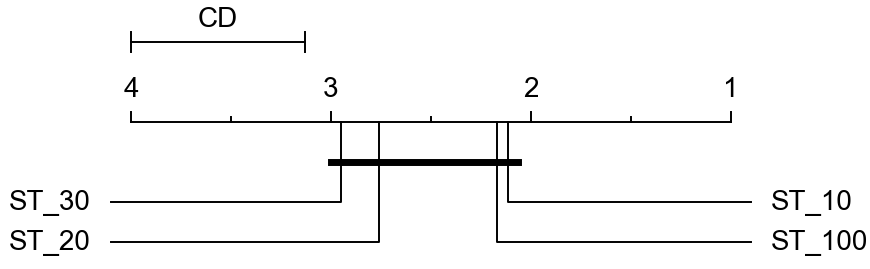
\includegraphics[width=0.49\textwidth]{cd_hm_within_st.png} & & 
    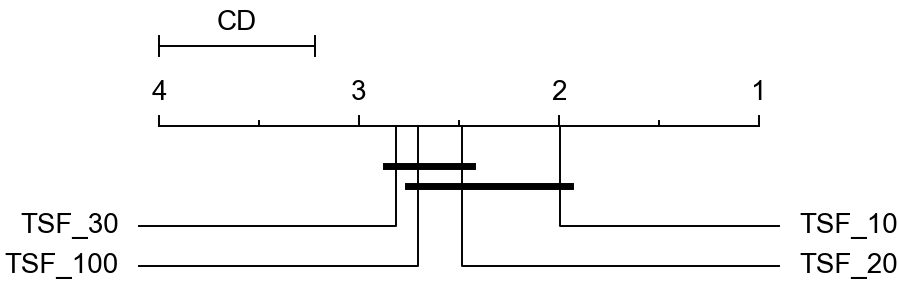
\includegraphics[width=0.49\textwidth]{cd_hm_within_tsf.png} \\
    \textbf{(c)} & & \textbf{(d)}  \\[6pt]
    \end{tabular}
    \begin{tabular}{ccc}
    & 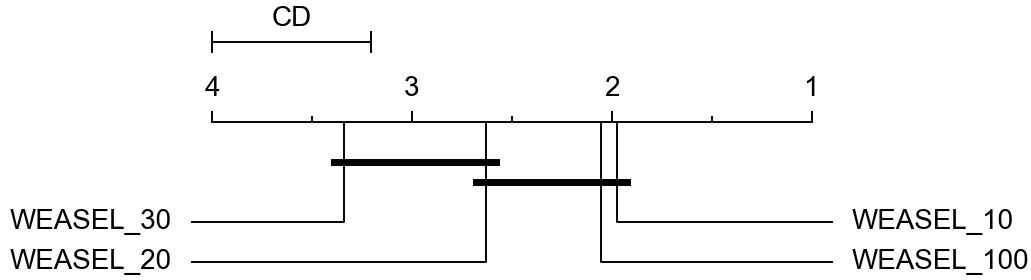
\includegraphics[width=0.49\textwidth]{cd_hm_within_weasel.png} & \\
    & \textbf{(d)} & \\[6pt]
    \end{tabular}
    \caption{ \textbf{(a)} CBoss
    \textbf{(b)} PForest
    \textbf{(c)} ST
    \textbf{(d)} TSF
    \textbf{(e)} WEASEL}
    \label{fig:within}
\end{figure}



Figure \ref{fig:within} shows the critical difference diagram for each classifier separately.
We compare each classifier on all the data sets that it finished across all the different chunks, regardless of the other classifiers.
The best performing algorithms lie on the right side of the diagram and the worse performing algorithms on the left side.
A bar is used to connect a clique of classifiers which are not significantly different based on their ranking. 

All classifiers show no significant difference between their 100\% classifier version and the 10\% version based on their $F_{\beta}-measure$ scores.
For CBoss, CBoss\_100 comes in the first place and CBoss\_10 comes in the second place. While for PForest, ST and WEASEL;
their respective 10\% versions; ST\_10, PForest\_10 and WEASEL\_10 rank first.
Although TSF shows no significant difference as well, but its 100\% version TSF\_100 comes in the third place.
The 20\% and 30\% versions for all the classifiers always show no difference in ranking.

If we switch to the critical difference diagrams of accuracies, we find rather different results.
For all the classifiers, the 100\% and the 10\% version are always significantly different in their ranking.
WEASEL\_100, CBoss\_100 and PForest\_100 are all significantly better than any of their other versions.
TSF\_100 and ST\_100 are ranked better than their 30\% versions TSF\_30 and ST\_30, but they are not significantly different.
This conforms with the concept of eTSC that as more data becomes available the better a classifier performs
and also demonstrates the role that earliness plays in the scores of $F_{\beta}-measure$.


\section{Results on Runtime Duration}
\label{SectionRuntime}
Another aspect we investigate for our experimentts is the runtime of the classifiers.
It is not possible to carry out a comparison between the different algorithms we have used; because of the different adaptations we have applied to them.
For some classifiers, have used an enhanced version which allows setting a contract time for feature extraction phases; like in the case of CBoss and ST.
This parameter allows us to restrict the amount of time given for the classifier.
For PForest, we have excluded two distance measures; euclidean distance because it cannot handle the early classifcation context
and TWE distance because it is the slowest elastic distance measure.
These enhancements make our results not representative for the original classifiers runtime performance.
Instead we provide information about the CPU time that was needed by each classifier to complete training on the data sets.
Table 1232346263458 shows the CPU time, in seconds, for all the classifiers on all the used data sets.
The values in the table represent the training time of the best model selected from the 5 cross validation folds.
If no cross validation was carried out, then the value represents the CPU time for the training process directly.
Failed runs and runs that exceeded the time constraint are excluded from the table.

Here should be a table

TSF and WEASEL have short training durations. TSF doesn't use any complex features and instead depends on simple summary statistics on intervals.
The stochastic selection of intervals speeds its learning process even faster.
WEASEL on the other hand is designed for speed and quality, but this comes on the expense of memory.
Although WEASEL takes short training times, it has failed to complete on some data sets due to its large memory print.
ST is known to be a strong but rather a significantly slow classifier.
The use of the contractable version of ST clearly pays off, it stabilizes the training time across the different chunks by limiting the time during which ST looks for shapelets.
The slowest classifier among all experiments was PForest. 

Please see Appendix (should mention appendix number or letter) for more information the breakdown of duration by length

Appendix (should mention appendix number or letter) for the breakdown of duration by train size

and Appendix (should mention appendix number or letter) for the breakdown of duration by number of dimensions

\section{Recommender Results}
\label{SectionRecommenderResults}
We divide our results for the recommender into two main parts. The firs part presents the results for the chunk learners, while the second part presents the results for the final recommendation of the whole recommender.
In the chunks learners results part, we discuss the performance of each chunk learner and the important features for building the random forests.
In the final recommendation part, we discuss the overall performance of the recommender based on its ability to correctly suggest good performing classifiers.

\subsection{Are the chunk learners able to learn F-scores for the classifiers ?}
\label{SubsectionFScoreResults}
% results for f-score
Table \ref{TableOverallErrors} shows the overall performance of the chunk learners across all 50 runs.
In general, the chunk learners are able to learn about the performance of classifiers on the different chunks, but their mean errors are relatively high.
As evident from the results, there is an inverse relation between the performance of the chunk learners and the revealed\%.
The chunk learner that trains on the 10\% results is able to score the best scores across all the chunk learners.
The more revealed data, the harder it becomes for the chunk learners to accurately predict performance of classifiers.

\begin{table}[hbt!]
    \setlength\extrarowheight{2pt} % for a bit of visual "breathing space"
    \begin{tabularx}{\textwidth}{|X|X|X|}
    \hline
    \textbf{Revealed\%} & \textbf{Avg MAE} & \textbf{Avg RMSE} \\ \hline
        10 & 0.048274974 & 0.067191131 \\ \hline
        20 & 0.095708094 & 0.124290807 \\ \hline
        30 & 0.120365517 & 0.154616709 \\ \hline
        100 & 0.155801376 & 0.195245175 \\ \hline
    \end{tabularx}
    \caption{Overall Performance of chunk learners over 50 runs}
    \label{TableOverallErrors}
  \end{table}

Figure \ref{Img:HistogramRMSE} gives a more detailed view of the distribution of RMSE for the chunk learners.
It is clear that not only the curves of the higher chunk learner shift towards higher error values, but also the spread of the values is wider.
This indicates that few of the predictions made by the lower chunk learner are significantly worse than their actual values.
While the higher chunk learner is generally worse and makes larger mistakes by predicting values that are clearly worse than the actual performance of the classifiers.

  \begin{figure}[!htbp]
    \captionsetup{justification=raggedright}
    \centering
    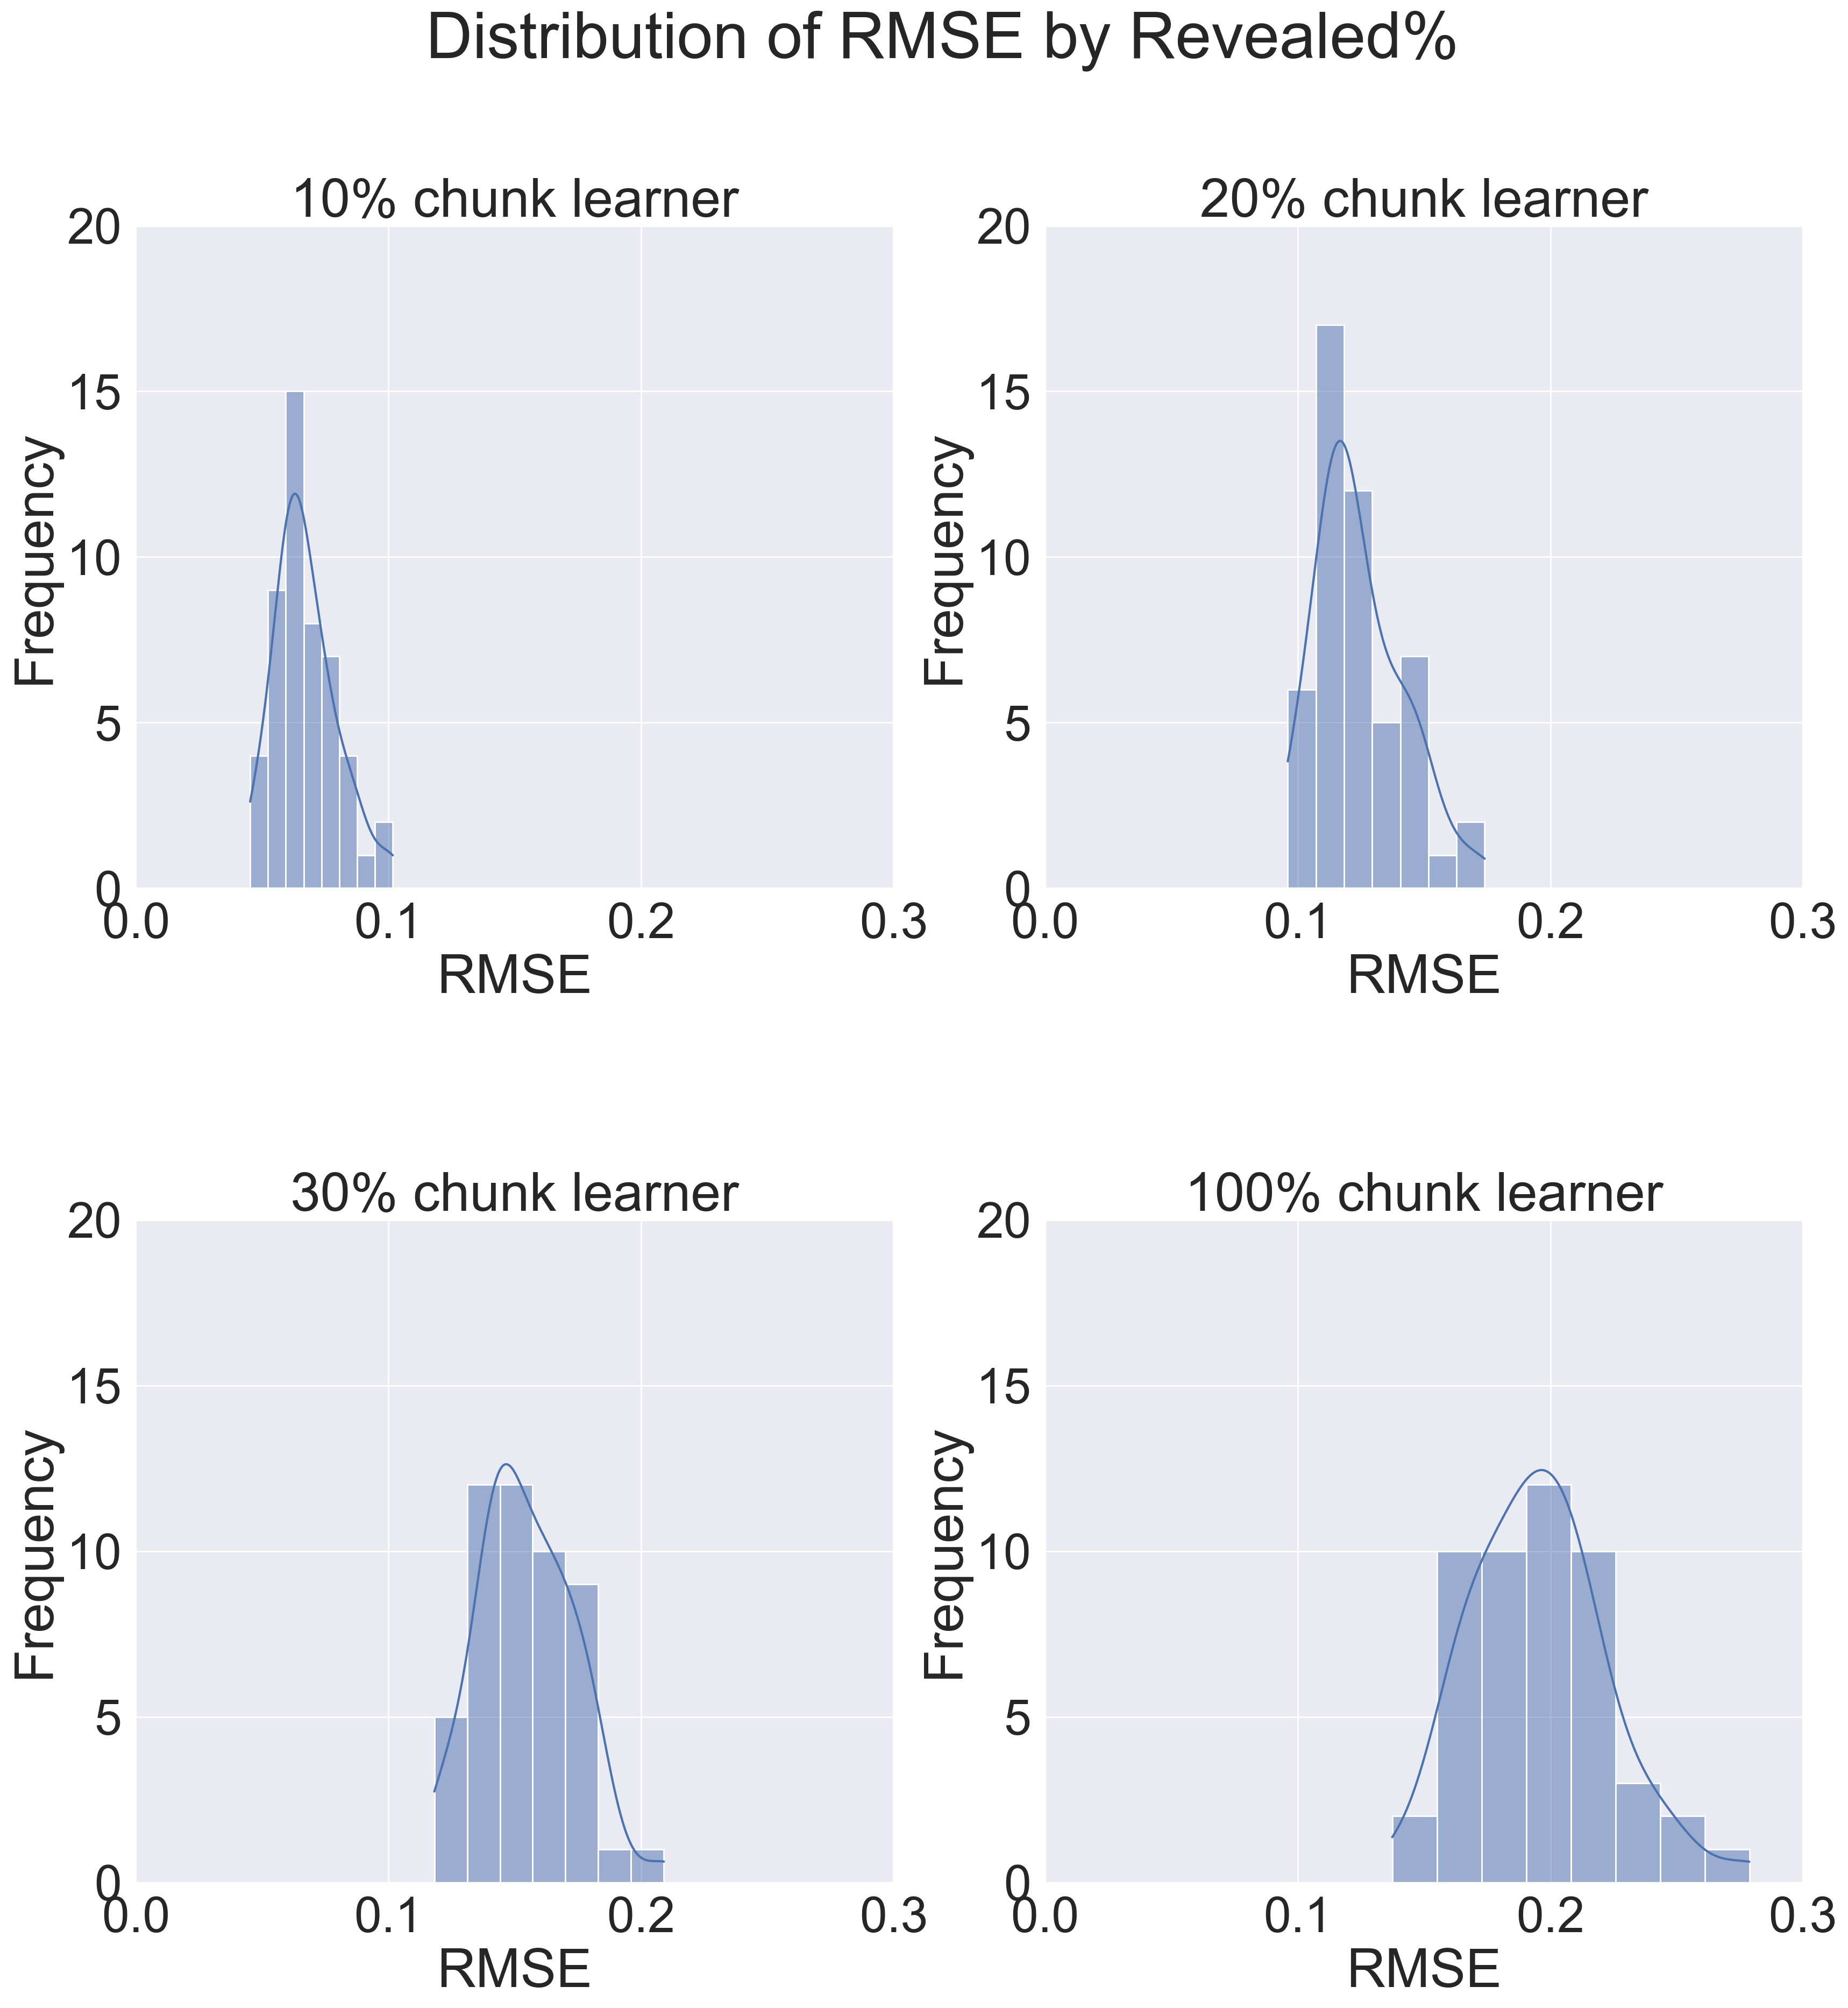
\includegraphics[width=\textwidth]{hist_rmse.jpg}
    \centering
    \caption{Histograms for distribution of RMSE per chunk over 50 runs}
    \label{Img:HistogramRMSE}
  \end{figure}

Figures \ref{Img:MAEClassifier} and \ref{Img:RMSEClassifier} visualize the MEA and RMSE of each chunk learner per classifier.
It is evident from the results that for CBoss, ST and WEASEL; the chunk learners are able to score better results as more data is revealed.
It is the opposite scenario for PForest. The first 3 chunk learners score the least errors for PForest, but on the 100\% dara the errors significantly increase to be the worst among all.
This explains the the long tail that appears in the 100\% chunk learner RMSE histogram due to the large differences between the actual and predicted F-scores for PForest on the 100\% data.

  \begin{figure}[!htbp]
    \captionsetup{justification=raggedright}
    \centering
    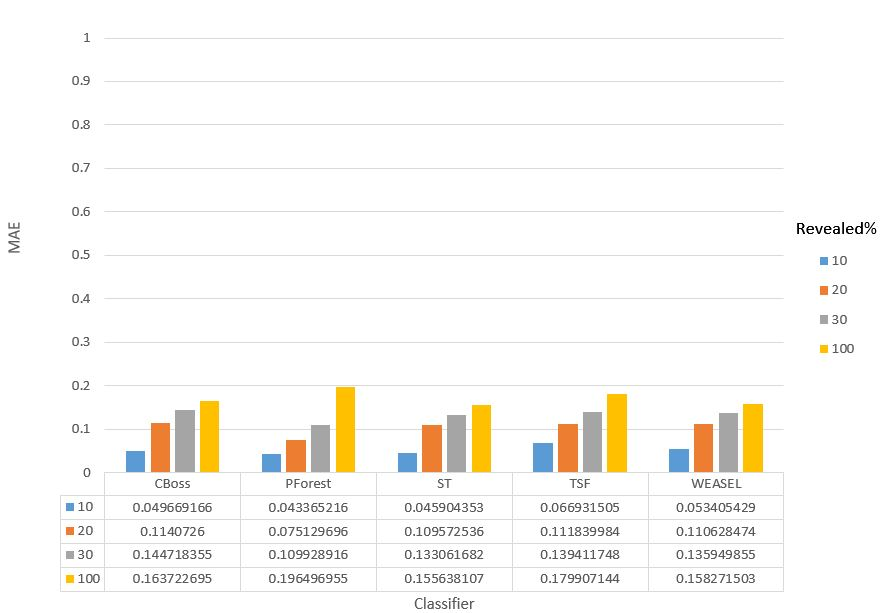
\includegraphics[width=\textwidth]{MAE_classifier.JPG}
    \centering
    \caption{Avg MAE for classifiers per chunk over 50 runs}
    \label{Img:MAEClassifier}
  \end{figure}

  \begin{figure}[!htbp]
    \captionsetup{justification=raggedright}
    \centering
    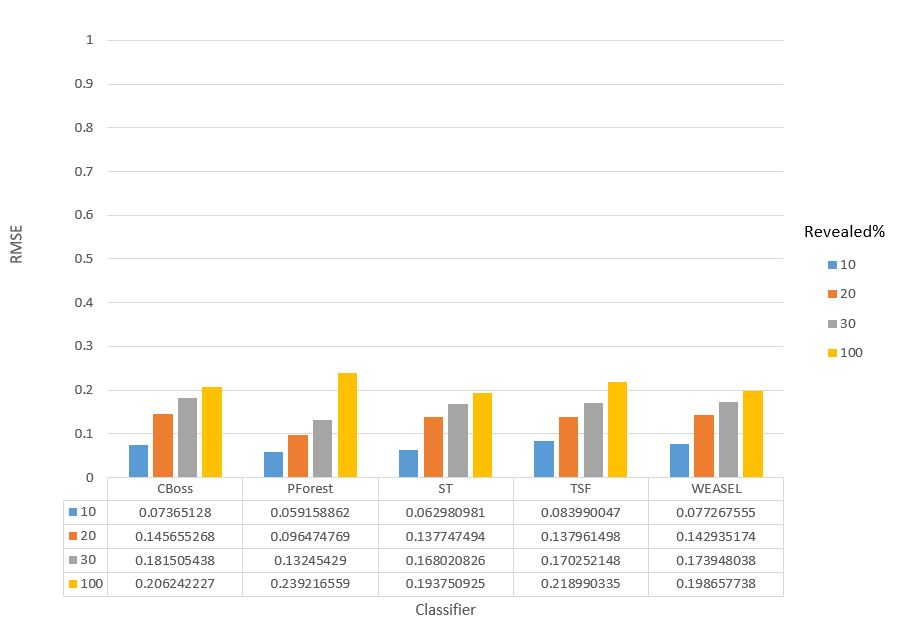
\includegraphics[width=\textwidth]{RMSE_classifier.JPG}
    \centering
    \caption{Avg RMSE for classifiers per chunk over 50 runs}
    \label{Img:RMSEClassifier}
  \end{figure}

\subsection{Which features contribute the most to the F-Score Prediction ?}
\label{SubsectionFeature}
% Feature importance
One of the main reasons why we chose to use random forests for the chunk learners, is that they give a notion of importance for features that were used to build the trees.
This helps understand what features play role in the prediction of scores for the classifiers for each chunk.

Figure \ref{Img:MeanFeatureImportance} shows the average importance of the features across all the 50 runs.
The feature importance is calculated using the default method from the $sklearn$ library; the mean decrease of impurity.
For each selected feature in the internal nodes of the regression trees, the impurity of the split is calculated using variance reduction.
After the whole forest is built, the mean variance reduction for each feature is calculated over all the trees.

\begin{figure}
    \captionsetup{justification=raggedright}
    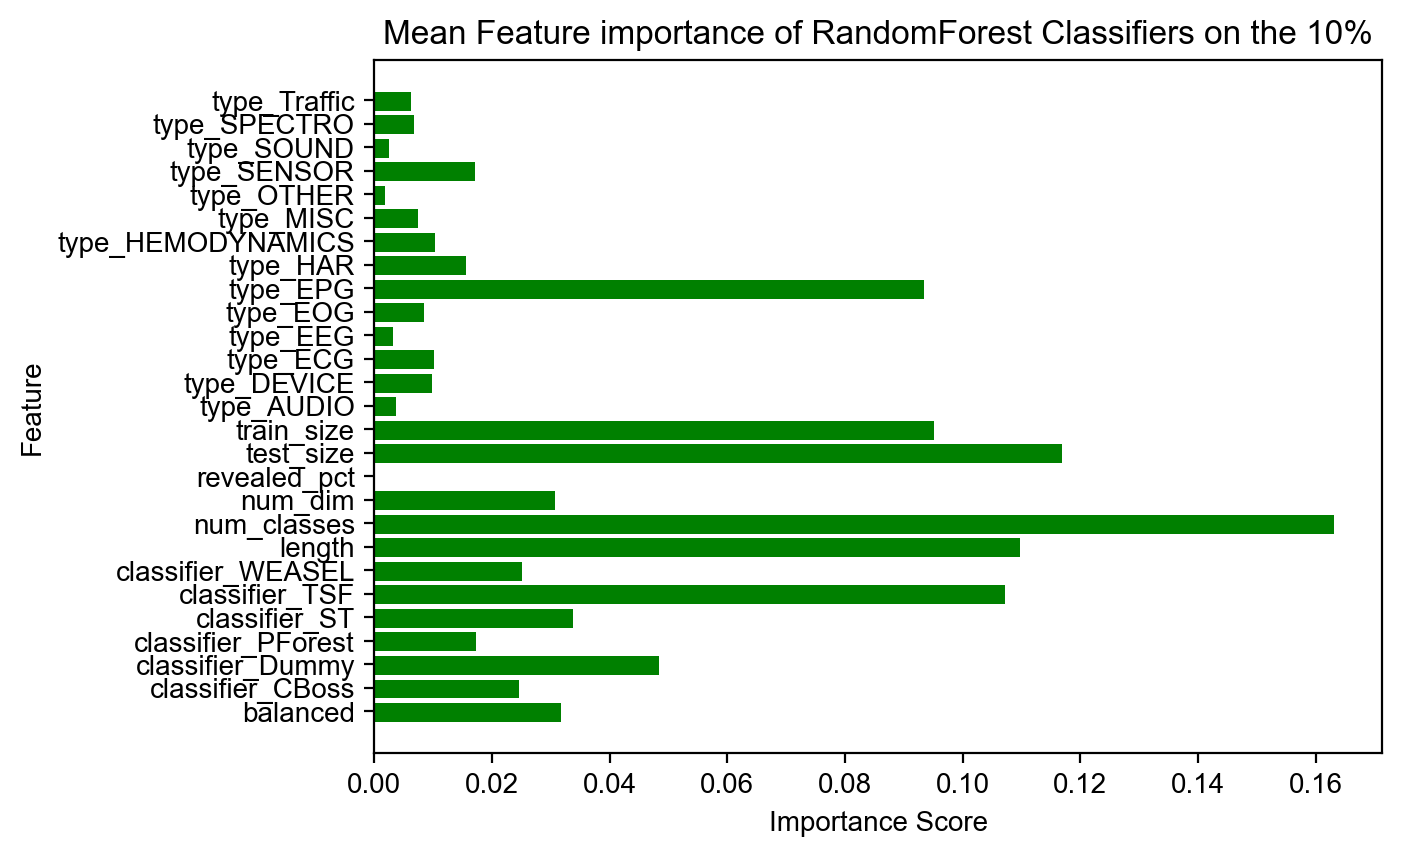
\includegraphics[width=0.49\textwidth,keepaspectratio]{mean_feature_imp_10pct.png}
    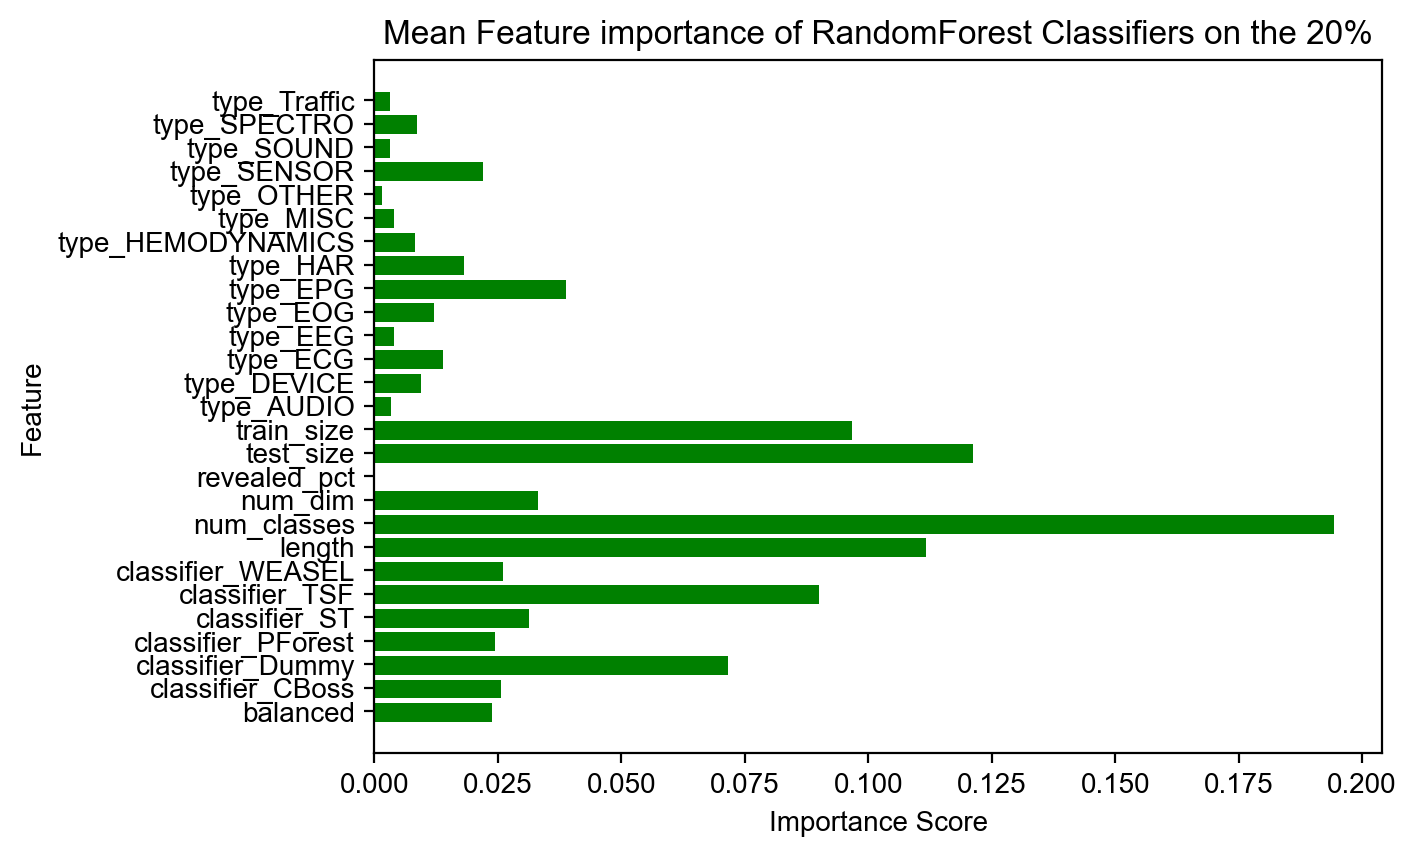
\includegraphics[width=0.49\textwidth,keepaspectratio]{mean_feature_imp_20pct.png}
    \\[\smallskipamount]
    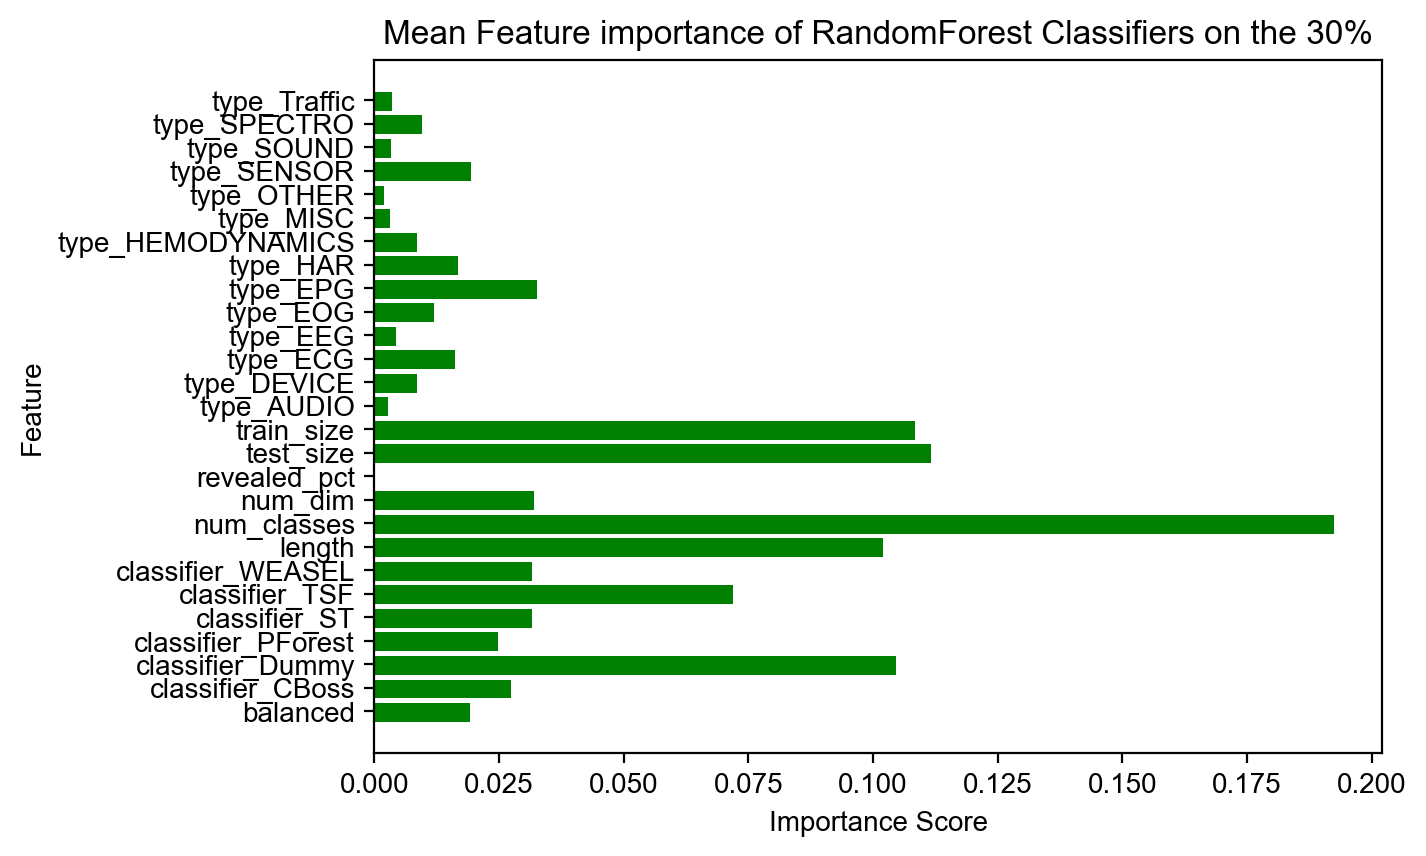
\includegraphics[width=0.49\textwidth,keepaspectratio]{mean_feature_imp_30pct.png}
    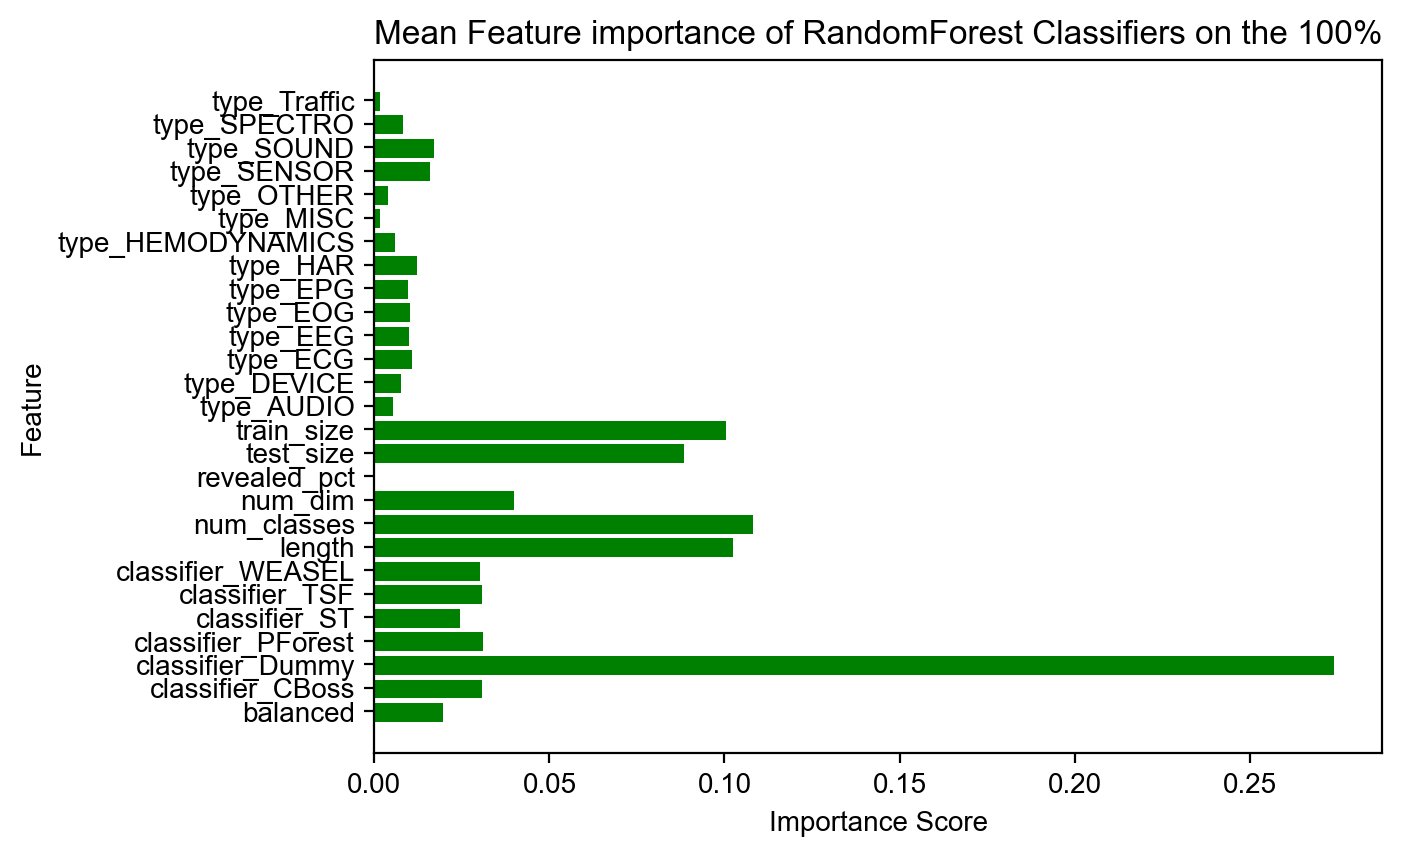
\includegraphics[width=0.49\textwidth,keepaspectratio]{mean_feature_imp_100pct.png}
    \caption{Mean Feature Importance per chunk across 50 runs}
    \label{Img:MeanFeatureImportance}
\end{figure}

For the lower chunk learners, the main metadata of the data sets; number of classes, length, train size and test size have the greatest importances among all the features.
The number of classes persistently has the highest feature importance over all other features.
It is also visible that TSF has high importance on the 10\% chunk results, which conforms with our CD diagram on the 10\% data; due to its significantly better performance.
This importance of TSF fades away as more data is revealed for the classifiers, while on the other hand the imoprtance of the dummy classifier increases.
For the 100\% chunk learner, the Dummy classifier has the highest importance.
This conforms with our results from the CD diagram from Figure \ref{fig:CDAcross},
where all the classifiers are much better than the Dummy classifier; which makes it easy to purely separate from all other results.
This then leads the importance of all the other classifiers to become closer to each other.

\subsection{Are the final recommendations of the framework consistent with actual results ?}
\label{SubsectionFinalRecommendation}
% results for final recommendation
In the end the final result of our framework is the recommendations of the recommender.

% avg accuracy

%  confusion matrix

% insight of the recall
It achieves a recall of 1 on the 100\% data. This indicates that on the full length data, the recommender never suggests a classifier which performs badly.
Although this is a quite impressive result, but we cannot contribute the score to the ability of the classifier to learn on the data.
From our CD diagrams results we know that the dummy classifier is significantly worse than all the classifiers on the 100\% chunk.
We also know that from the F-Score results that the chunk learner on the 100\% data has the highest average RMSE values across all the runs and it makes predictions which are 
Thus, we believe that the reason such a high score is achieved; is because the dummy classifier is the baseline that decides whether a certain classifier is good or bad.
The dummy classifier is a very weak classifier and allows for a wide span of error without affecting the results of the recommendation.